\documentclass{article}
\usepackage{multicol}
\usepackage{longtable}
\usepackage{caption}
\usepackage{booktabs}
\usepackage{array}
\usepackage{multirow}
\usepackage[super,sort&compress]{natbib}
\usepackage[margin=1in]{geometry}
\usepackage{graphicx}
\usepackage{float} 
\usepackage{url}
\usepackage{ragged2e}
\usepackage{siunitx}

\title{From Memory Loss to Mastery: Procedural Learning in Transient Epileptic Amnesia and Frontal Encephalomalacia Post Traumatic Brain Injury}
\author{Benjamin Kane BSc.}

\begin{document}

\maketitle

\section*{Abstract}
This autoethnographic study explores the lived experience of neurological multimorbidity, including obstructive hydrocephalus, traumatic brain injury, frontal encephalomalacia, dysexecutive syndrome, and transient epileptic amnesia. Integrating personal narrative with clinical data, neuroimaging, neuropsychological assessments, and psychiatric treatment, it documents a life shaped by invisible intersecting neurological conditions.

Central to this narrative is the disruption and partial reconstruction of autobiographical memory and executive function following prolonged misdiagnosed traumatic brain injury and delayed neurosurgical intervention. Marked by emotional trauma, substance abuse, academic excellence, and professional resilience, these medical crises illustrate the interplay between impairment and resilience.

This first-person account challenges reductive biomedical narratives highlighting cognitive, emotional and social dimensions of chronic neurological illnesses. It argues that neurological multimorbidity, though often hidden, exerts a profound effect on identity, self-regulation and social inclusion. Through methodological reflection and structured adaptation, it demonstrates that neurodivergent functioning can coexist with cognitive resilience, offering insight for clinicians, researchers and neurodivergent individuals navigating complex neurological conditions.

\section*{Keywords}
autoethnography, neurological multimorbidity, obstructive hydrocephalus, tectal glioma, frontal encephalomalacia, transient epileptic amnesia, dysexecutive syndrome, neuropsychology, neuropsychiatry, addiction, neuroplasticity, procedural learning, cognitive compensation, cognitive rehabilitation

\section*{Introduction}
Undiagnosed neurological conditions can profoundly disrupt a person’s sense of time, identity and continuity. The body’s capacity to adapt to chronic dysfunction, often silently, enables continued functioning, but frequently masks underlying pathology. This quiet endurance may create an illusion of “normal” life, even as cognitive and emotional deterioration progresses beneath the surface.

This study explores one such case. Beginning in adolescence, I experienced a progressive decline in autobiographical memory, ultimately leading to a diagnosis of hydrocephalus caused by tectal glioma. I regained consciousness on December 30th, 2008, at the Royal Free Hospital in Hampstead Heath, with no recollection of how I had arrived or what had preceded my admission. A programmable ventriculoperitoneal (VP) shunt was inserted, draining excess cerebrospinal fluid from my third ventricle into my abdomen. My life had been saved, though at a significant cognitive and emotional cost.

This study responds to the gap in literature surrounding the lived experience of complex, overlapping neurological conditions. Through autoethnographic methods, it seeks to bridge biomedical psychological and narrative understandings of memory loss, identity disruption and recovery. By integrating clinical data with first person reflection, it offers a perspective often absent from conventional neurological and neuropsychological discourse.

\section*{Methods}
This study adopts an analytical autoethnographic approach, in which the author serves as both the subject and researcher. Autoethnography provides a framework for investigating the lived experience of neurological multimorbidity through critical self-reflection, integrating personal narrative with clinical documentation. This method enables the examination of how memory, identity and cognitive function are shaped by intersecting
neurological conditions, including hydrocephalus, dysexecutive syndrome, transient epileptic amnesia and associated psychiatric comorbidities.

Data sources include reconstructed autobiographical memory, elicited through conversations with close friends and family, as well as clinical documentation such as MRI scans, neurosurgical records and comprehensive neuropsychological and neuropsychiatric assessments.

Verbal consent was obtained for all contributory conversations. These external accounts were used to corroborate and contextualise fragmented inaccessible autobiographical memory.

This approach systematically explores the impact of memory loss, social disruption and cognitive dysfunction, examining how achievements and adaptive capacities emerged despite chronic neurological multimorbidities. The methodology aims to interpret the long-term consequences of undiagnosed traumatic brain injury resulting from obstructive hydrocephalus, while identifying the compensatory strategies developed in response.

\section*{Patient Or Public Contribution}
As patient and author, I led this autoethnographic study, providing first-person reflections on living with neurological multimorbidity focusing on identity, memory and recovery. My lived experience forms the core narrative, exploring the impact of memory loss, social disruption and personal achievements including a 1st class degree and succeeding professionally as a software engineer, shaped by long-term undiagnosed hydrocephalus.

Contributions from family and close friends, such as father’s hospital advocacy, grandmother's 2024 accounts and close friends reconstructed fragmented memories, offering external perspectives enhancing authenticity. These contributions did not influence structure or analytical framework, but supported its validity by corroborating key events and experiences.

\section*{Early Life}
I was raised by a single father alongside my older brother and sister. Throughout my childhood, life appeared typical and stable, but at the age of twelve or thirteen, changes emerged. Returning from school, I often found myself unable to stay awake, sleeping for several hours at a time. In retrospect, this may have been the beginning of my underlying neurological conditions.

Symptoms subsided temporarily but returned around the age of sixteen with greater severity, marking the onset of my underlying neurological condition.

\section*{Headache And Adaptation}
The first major symptom was the onset of intense, relentless headaches - so severe that I unconsciously adapted how I moved. I recall a friend, whose family would play a vital role in caring for me during my decline, once asking:
\begin{center}
“Why do you turn your whole body instead of your head”
\end{center}

I hadn’t realised I was doing this. I instinctively stopped moving my head as any motion would trigger unbearable pressure – pain so intense it often resulted in loss of consciousness. A survival response to an invisibly escalating neurological threat.

\section*{Incontinence And Motor Decline}
The next symptom was incontinence. I could not choose when I wanted to go to the toilet, it chose for me. There are documented instances of incontinence including during work hours which contributed to social withdrawal and embarrassment. It also occurred during sleep.

Then came loss of motor control. I began dragging one side of my body, as if I had suffered a stroke. This physical decline is unmistakable to others, yet still without definitive diagnosis.

\section*{Cognitive Decline And Social Collapse}
As cognitive function progressively deteriorated, I failed my A levels and subsequently applied for college. This coincided with being forced to leave home, initiating a period of acute personal and neurological instability. The severity of headaches during this time is difficult to articulate with conventional clinical or experiential framework. My levels of consciousness deteriorated at an exponential rate.
\begin{center}
The severity of headaches defies comparison. There is no adequate measure for that level of pain.
\end{center}

\section*{Final Memory Before Diagnosis}
With much of my memory lost, my final recollection is of my father. He called and said:
\begin{center}
    “Ben something’s wrong, pack a bag, I’m taking you to hospital”
\end{center}

\noindent That was it.\\
\\
Following an initial assessment I was deemed medically stable and ready for discharge. It was only when my father insisted on a more thorough examination. A scan was performed and subsequently I was transferred to The Royal Free Hospital – diagnosed with obstructive hydrocephalus caused by tectal glioma. My first ventriculoperitoneal (VP) shunt was fitted.

\begin{figure}[H] 
\centering


\includegraphics[width=0.9\textwidth]{figure table.png}
\caption*{Figure 1 - 3 provide an overview of MRI findings in chronic obstructive hydrocephalus secondary to tectal glioma, including pre- and post-shunting images and the tectal lesion (2008--2018).}
\label{fig:mri-overview}
\end{figure}

\section*{Rebuilding Lost TIme}
The autobiographical memory deficit, caused by undiagnosed hydrocephalus appeared profound in its initial presentation. However, through autoethnographic reflection and conversations with others, fragments of my past have been partially reconstructed, revealing the extent to which my condition disrupted both memory and identity. 

In 2024, my grandmother recounted an incident on August 28, 2008 - 125 days before my diagnosis. While preparing to attend the Reading Music Festival, my frequent visits to London for such events had masked my deteriorating health, sustaining an illusion of normalcy. Yet, that day my lethargy and disengagement prompted her frustration. She recalled sitting at the top of her stairs, head in hands, initially attributing my behavior to substance abuse - a misinterpretation echoing the social stigma often faced by those with undiagnosed neurological symptoms. 

Her account triggered the vivid image of her sitting head in hands. However the journey to Waterloo Station remains absent, underscoring the persistent gaps marking the worsening of my condition. 

She later recalled observing me walking “like an old man”, a manifestation of motor decline akin to the earlier adaptations I made to severe headaches and hemiparesis. This marked a shift in her perception, recognising my symptoms as pathological rather than self-inflicted. This account, like my father’s insistence on a thorough hospital evaluation, underscores the critical role of external perspectives in illuminating my condition. 

Reconstructing these lost moments through the narratives of others parallels the surgical intervention of the ventriculoperitoneal shunt, both attempts to restore what was disrupted. Yet, this process remains incomplete, reflecting the ongoing negotiation of identity and recovery in the context of neurological multimorbidity.

\section*{Shunt Failure, Encephalitis And Further Memory Loss}
In August 2009, less than a year from initial diagnosis of hydrocephalus and ventriculoperitoneal shunt placement, I developed symptoms suggestive of shunt failure, including chronic idiopathic constipation, severe headaches and disorientation. This prompted a brief admission to the local Accident and Emergency department. Memory fragmentation resumed.

Following discharge I attended Reading Music Festival again in 2009, however due to complications attributed to shunt failure I have no recollection of this event, only photographs. Secondhand accounts describe my disoriented state post-festival. I arrived at the home of a family who had cared for me before my 2008 diagnosis and slept on their sofa. Early the next morning, I walked barefoot through the snow to my father’s house, where a neighbor found me and returned me to my residence.

When my father visited, he found me unresponsive, prompting another emergency admission. Assessed with the Glasgow Coma Scale, I scored 8, indicating severe neurological impairment consistent with shunt failure. I was transferred to the Royal Free Hospital, where my ventriculoperitoneal shunt was removed and replaced with an External Ventricular Drain (EVD). During this period, I reportedly fell, dislodging the first EVD, necessitating a second surgery.
\\
\noindent
\begin{minipage}[t]{0.30\textwidth}
  \vspace*{-2pt}
  \centering
  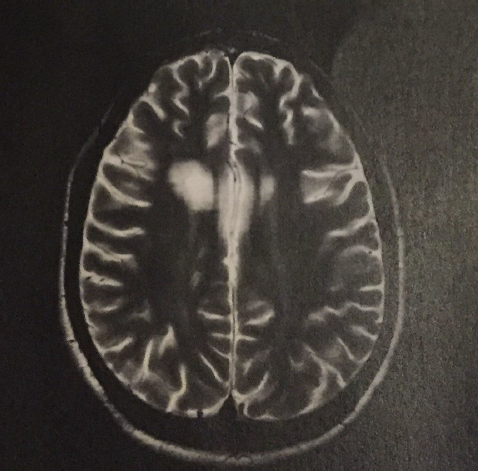
\includegraphics[trim=0 0 0 0,clip,width=0.85\linewidth]{Frontal encaph.png}
  \small\itshape
  Figure 4. T2-axial MRI showing right frontal encephalomalacia post-EVD
  \label{fig:frontal-encephalomalacia}
\end{minipage}
\hfill
\begin{minipage}[t]{0.65\textwidth}
\vspace{2pt}
After weeks of treatment for infection, I regained consciousness. However the EVD placement in the right lateral ventricle caused right frontal encephalomalacia as seen in figure 4. This softening and loss of brain tissue resulted in permanent cognitive and emotional impairments that remain largely invisible to others.

\vspace{3mm}
The hidden nature of encephalomalacia’s consequence causes an isolated impact of neurological multimorbidity, complicating recovery and social reintegration.
\end{minipage}

\section*{Onset Of Neurological Symptoms During University}
Following the 2009 shunt failure and resultant encephalomalacia, I commenced a Computer Science degree at the University of Hertfordshire, achieving a 1st class grade in my first year. Beneath this achievement, new neurological symptoms emerged, further disrupting my autobiographical memory and sense of self.

On 3rd December 2010, during a Pendulum concert at Wembley Arena, I experienced my first olfactory hallucination, an indescribable smell. This was followed by vivid auditory and experiential hallucinations including the band saying something similar to “Don’t worry about the smell, we’re trying something”. In retrospect, this episode was likely my first seizure.

Towards the end of my first year at university, around May 2011, these episodes became more prominent and observable. During these episodes, autobiographical memory lapsed entirely, producing disorienting temporal gaps. I was admitted to the Queen Elizabeth II Hospital in Welwyn Garden City.

The seizures had progressed into déjà vu-like events, where I would ask the same question repeatedly, each time forgetting what I had just asked. Vacant stares and unresponsiveness to those around me became another prominent symptom. I was later discharged, without diagnosis.

\section*{Summer 2011}
During the summer following completion of my first year at university, the frequency and intensity of episodes increased. particularly upon waking. During this period, working night shifts through an oppressive summer heat, temporarily living at my sister’s and sleeping on her sofa, directly facing the sunrise. Fragmented sleep and disorientation became the norm.

One episode remains explicitly vivid. Waking disorientated during early hours of the morning, I left the flat, running repeatedly between two floors. I could recall the five-digit access codes for each floor - one of which I had used only once - yet unable to remember the door I was staying behind. The cycle continued several times until becoming more alert and returning to my sister's home. Later that day fragments of autobiographical memory began to reassemble.

Similar patterns occurred whilst at my partner’s home in Debden, Essex, between shifts. I would wake confused, repeatedly asking the same questions while forgetting what I had asked. These episodes exemplified how disorientation became routine - yet remained invisible to others. Eventually I returned to the neurosurgical team and was referred to neurology for further investigation with suspicion of an epileptiform cause.

\section*{Diagnosis - Transient Epileptic Amnesia}
Following referral to the neurological team, an electroencephalogram (EEG) revealed abnormal electrical activity localised in the left temporal lobe, specifically involving to the left hippocampus. This resulted in a diagnosis of transient epileptic amnesia (TEA), characterised by recurrent amnesic episodes affecting autobiographical memory, distinct from earlier shunt failure and undiagnosed hydrocephalus.\cite{zeman1998,butler2007}

The hippocampi, two critical structures within the limbic system of the brain's left and right hemispheres, are essential for verbal and spatial memory. The left hippocampus supports verbal processing and recall (including words, terms and conversations), autobiographical memory (the recollection of past personal events), contextual memory (associating events and locations) and memory consolidation (the transfer of information from short-term to long-term memory).\cite{squire1992,burgess2002}.

Learning and retaining new information is not just disrupted during these epileptic episodes but also in everyday functioning. This hidden impairment adds a complex layer to my neurological multimorbidity, complicating social engagement, personal development and academic progress.\cite{squire1992,zeman2010}

The diagnosis of TEA marked a significant new phase in my memory challenges, distinct yet compounding the deficits from undiagnosed hydrocephalus and shunt failure in 2009. This episodic amnesia and associated cognitive dysfunctions further hindered social engagement, learning and distinct behaviours, amplifying the multifaceted impact of neurological multimorbidity.\cite{zeman2010,miskin2020}

\section*{Treatment}
Following the 2011 diagnosis of TEA, distinct from 2009 shunt failure and erased memories like the Reading Music Festival, I was initially prescribed Levetiracetam to control seizures. However, side effects, including xerodermia (predominately affecting hands, eyes and lips) and chronic fatigue, significantly impacted my quality of life, restricting social engagement and personal development\cite{patsalos2000,mula2013}. Due to persistent seizures and debilitating side effects, Levetiracetam was discontinued in favor of Carbamazipene, reducing seizure frequency.

Subsequently, I transitioned to a combination of Lamotrigine (250mg mane, 300mg nocte, later reducing to 275mg nocte) and 800mg Sodium Valproate - (Epilim Chrono) bd. Seizures were controlled until Epilim was discontinued due to reducing polypharmacy as additional multimorbidity conditions were diagnosed. Subsequently, Cenobamate (200mg nocte) was introduced, a medication for patients with refractory epilepsy, unresponsive to multiple antiepileptics.\cite{french2020}

\section*{Neuropsychology}
Due to ongoing concerns regarding memory impairment, attention difficulties and the cumulative impact of multiple neurological multimorbidity, a referral was made by neurology for a comprehensive neuropsychological evaluation. The assessment, lasting 3.5 hours, was made to assess cognitive strengths and weaknesses and clarify reported memory difficulties.

A battery of standardised neuropsychological tests compensating for traumatic brain injury and epilepsy were conducted. These included the Wechsler Adult Intelligence Scale - Fourth Edition (WAIS-IV), the Brain Injury Rehabilitation Memory and Information Processing Battery (BIRT- BMIPB), and Delis-Kaplan Executive Function System (D-KEFS).

\section*{Memory}
BIRT-BMIPB was used to assess both verbal and visual memory - areas impacted by my long term hydrocephalus and subsequent neurological conditions. This enabled insight into the extent and profile of memory impairment, helping to differentiate between retrieval and encoding deficits, areas commonly affected by neurological multimorbidity.

\begin{table}[htbp]
\centering

\caption{Verbal memory performance (BIRT-BMIPB)}
\label{tab:verbal-memory}

\begin{tabular}{
  >{\RaggedRight}p{7.8cm}
  >{\centering\arraybackslash}p{2.8cm}
  >{\centering\arraybackslash}p{4.2cm}
}
\toprule
\textbf{Task} & \textbf{Score} & \textbf{Range} \\
\midrule
Recognition Memory Test for words      & 49/50 & \textgreater75th percentile \\
Story Recall - immediate               & 16/60 & 10th percentile \\
Story Recall - delayed                 & 16/60 & 10--25th percentile \\
List Learning - immediate              & 46/75 & 10--25th percentile \\
List Learning - recall after distractor& 10/15 & 25th percentile \\
\bottomrule
\end{tabular}
\end{table}
\begin{table}[htbp]
\centering

\caption{Visual memory performance (BIRT-BMIPB)}
\label{tab:visual-memory}
\begin{tabular}{
  >{\RaggedRight}p{7.8cm}
  >{\centering\arraybackslash}p{2.8cm}
  >{\centering\arraybackslash}p{4.2cm}
}
\toprule
\textbf{Task} & \textbf{Score} & \textbf{Range} \\
\midrule
Camden Topographical Memory Test &
25/30 &
20--50th percentile \\
Figure Recall - immediate &
59/80 &
10--25th percentile \\
Figure Recall - delayed &
50/80 &
10--25th percentile \\
Doors \& People - Shapes &
33/36 &
35th percentile \\
\bottomrule
\end{tabular}

\end{table}

As shown in \textbf{Table 1} and \textbf{Table 2}, verbal learning and recall were moderately impaired while visual episodic memory showed mild to moderate underperformance. These deficits significantly impair the acquisition and retention of new information. Such challenges are further exacerbated by broader cognitive and emotional consequences of neurological multimorbidity.

In daily life, these impairments manifest in fragmented conversations, forgotten instructions and a persistent sense of disconnection from both social and professional contexts. This further illustrates how recognition, triggered by seeing or hearing key identifiers, provides a necessary prompt for memory retrieval. Learning new information, whether it be a name, location or professional routine requires structured repetition and consistent reinforcement to compensate for impaired memory consolidation and retrieval. This aligns with established neuropsychological models highlighting the role of both the hippocampus and frontal lobes in contextual and working memory processing.\cite{eichenbaum2017,stuss2000} These strategies serve to offset memory deficits in encoding and retrieval, compounded by broader cognitive consequences of neurological multimorbidity.\cite{lezak2012,feinstein2011} 

Paradoxically, the use of compensatory strategies allowed me to master complex skills, such as mastering Rubik’s cubes and working effectively as a software engineer. Through these adaptations, compensating for cognitive impairment illustrates how intellectual capacity, autobiographical and semantic memory can effectively coexist within a dynamic environment.

Visual perception and visuospatial skills were intact, reinforcing the aspect of recall and retention of new information deficits, over active working memory.

\section*{Executive Function}
% Replace your current Executive_Function content (or inline table) with this:

To assess executive cognitive skills, subsets of the D-KEFS were used, specifically Letter Fluency, Category Fluency, and Category Switching. These tasks evaluate verbal productivity, mental flexibility, and the ability to shift between semantic categories — core components of executive functioning. \textbf{Table 3} presents the age-based fluency scores obtained at age 25, which fell in the superior (scaled 14–15) to very superior (16+) ranges.

\begin{table}[htbp]
\centering
\caption{D-KEFS verbal fluency scores at age 25}
\label{tab:d-kefs-fluency}

\setlength{\tabcolsep}{8pt}
\renewcommand{\arraystretch}{1.12}

\begin{tabular}{
  >{\RaggedRight}p{7.8cm}
  >{\centering\arraybackslash}p{1.6cm}
  >{\centering\arraybackslash}p{2.0cm}
  >{\centering\arraybackslash}p{2.8cm}
}
\toprule
\textbf{Task} & \textbf{Raw Score} & \textbf{Scaled Score} & \textbf{Percentile Rank} \\
\midrule
Letter Fluency -- `FAS' (words in one minute)   & 58 & 16 & top 2\% \\
Category Fluency -- Animals and Boys (names in one minute) & 61 & 19 & top 0.1\% \\
Category Switching -- Fruits and Furniture (in one minute) & 18 & 15 & top 5\% \\
\bottomrule
\end{tabular}
\end{table}

During the assessment, the neuropsychologist described these scores as exceptional and rarely observed in clinical practice. Despite expectations of reduced performance due to my history of neurological multimorbidity, I demonstrated unexpectedly high levels of executive functioning, challenging those predictions.

\section*{Speed And Attention}
Auditory attention and working memory were assessed using the WAIS-IV digit span sub test. Interestingly, it was noticed that performance improved with task complexity, six digits forward, five backwards and seven sorted. This resulted in a composite score 11, placing in the average range.

Processing speed was assessed using WAIS-IV Symbol Search subtest. This assesses visual-motor speed, concentration and accuracy, resulting in a score of 12, indicating high average.

When compared to earlier verbal and visual memory tests, this reflects the complexity of retained cognitive strengths and practical difficulties in daily life. Difficulties with fragmented conversations, following instructions and social or professional disconnection highlight continued functioning impact.

\section*{Dysexecutive Syndrome}
A diagnosis of dysexecutive syndrome was made, characterised by impairments in behavioural inhibition, increased impulsivity, irritability, distractibility and perseveration. The symptoms are consistent with frontal lobe dysfunction and associated encephalomalacia as observed with neuroimaging, attributed to long standing hydrocephalus and secondary injury following shunt failure and EVD placement.

Living with dysexecutive syndrome, is at times, like not having that little voice in your head telling you whether it is appropriate to do or say something. A crucial cognitive construct underpinning both social and professional environments. As an invisible misunderstood impairment, it creates significant difficulties in interpersonal situations and emotional responses, often resulting in negative or unintended consequences, making it difficult to sustain long term relationships and stable employment.

\section*{Learning With Transient Epileptic Amnesia And Dysexecutive Syndrome}
Due to lapses in concentration and deficits in both visual and verbal memory, the ability to retain new information is significantly impaired. Frontal lobe encephalomalacia further compromises cognitive functions, most notably in processing and learning new information and sustaining attention, particularly when grouped with TEA. This frequently results in becoming hyperfocused or easily distracted, often resulting in missed or fragmented information. Impaired impulse control and executive dysfunction often results in behavioural dysregulation and inappropriate and antisocial outbursts when cognitively overloaded or distracted.

Long term learning and retention, particularly through lived experience, can be effectively supported through structured repetition and reinforcement. Being able to sustain attention and recall new information is significantly compromised due to this form of epilepsy. It is common to become distracted or fixate on earlier parts of conversations leading to loss of subsequent context. Clear written instructions and personal engagement to reinforce content are essential compensatory strategies, offsetting deficits associated with dysexecutive syndrome.

Strategies for retaining long term information can be effectively implemented through repeating tasks to reinforce the learning. Breaking down tasks into smaller manageable components supports attention and processing, a process often impaired by frontal encephalomalacia and temporal lobe epilepsy, particularly with abnormal hippocampal functioning. This structured incremental approach offsets attention deficits improving consistent learning outcomes.

This is evident by progressive mastery of increasingly complex Rubik’s cubes, a cognitively demanding task requiring the acquisition and application of multiple algorithms determined by visual and spatial reasoning. Through repeated engagement, these patterns gradually transitioned into procedural, or muscle memory. This enabled more fluid executions despite underlying memory deficits. \textbf{Table 4} compares the complexity of these puzzles in terms of piece counts, total possible arrangements, and puzzle types. 

Whilst progressing onto more advanced puzzles, such as the Master Cube (4x4) and Professor Cube (5x5), new algorithms are not only learned, but integrated with those in simpler versions. This cumulative process structured recall and sequencing of strategies. The complexity increased further with puzzles like the Megaminx and Gigaminx, dodecahedron shaped variants, introducing additional spatial dimensions and algorithmic depth. This furthermore adds higher level visuospatial manipulation and executive control.

Solutions were acquired through written guides and instructional videos, with each step segmented into discrete algorithmic categories. Mastery was achieved through repeatedly mixing and execution of the algorithms until they could be fully committed to procedural memory. These strategies exemplify compensatory strategies for managing visual and verbal memory deficits, reinforcing learning through structured repetition and incremental challenges.

\begin{table}[H]
\centering

\caption{Puzzle Complexity}
\label{tab:puzzle-complexity}

\setlength{\tabcolsep}{8pt}
\renewcommand{\arraystretch}{1.12}

\begin{tabular}{lrrrrr}
\toprule
\textbf{Type} & \textbf{Pieces} & \textbf{Arrangements} & \textbf{Centers} & \textbf{Edges} & \textbf{Corners} \\
\midrule
Rubik's 3×3 cube          & 26  & \num{4.33e19}   & 6   & 12 & 8 \\
Master 4×4 cube           & 56  & \num{7.4e45}    & 24  & 24 & 8 \\
Professor 5×5 cube        & 98  & \num{2.83e74}   & 54  & 36 & 8 \\
Megaminx (dodecahedron)   & 62  & \num{1.01e68}   & 12  & 30 & 20 \\
Gigaminx (dodecahedron)   & 242 & \num{3.65e263}  & 132 & 90 & 20 \\
\bottomrule
\end{tabular}
\end{table}

Procedural learning relies on the neural circuits within the basal ganglia and motor cortex, which remain relatively preserved despite neurological atrophy, providing a distinct adaptive pathway.\cite{doyon2005,peterson2016} Structured incremental repetition of complex tasks enhances synaptic plasticity despite visual episodic deficits in memory.\cite{kandel2014} These principles align with utilising intact procedural memory compensating for declarative memory impairments.\cite{squire2004,vakil2005}

Applying these strategies during my academic studies led to measurable improvements as evidenced in my programming modules by progressing from 61\% in semester A to 87\% in semester B during my first year at university. This demonstrates the adaptability and efficacy of structured procedural learning. It is also evident that as tasks increase in complexity, dysfunctional behaviours become more pronounced, manifesting in heightened frustrations, emotional dysregulation and impulsivity. These challenges often contributed to social disengagement and persistent difficulties in the workplace. Impulsive responses, without having that “little voice in your head”, frequently manifested in awkward interactions with colleagues, increasing the likelihood of interpersonal conflict and workplace tension.

Inner speech plays a critical role in self-regulation and impulse control, core aspects of dysexecutive syndrome. Internal verbal monitoring associated with heightened impulsivity and reduced execution control, as demonstrated in experimental paradigms where blocking of the inner voice, led to more impulsive behaviour.\cite{tullett2010}

\section*{Structured Programming As Cognitive Compensation}
To manage cognitive impairments stemming from executive dysfunction, structured programming frameworks offer an effective way to mitigate associated challenges with dysexecutive symptoms. In particular Test Driven Development (TDD) and Behavioural Driven Development (BDD) provide a cognitive scaffolding that supports task management, sustained focus and reduced mental fatigue.\cite{beck2003,janzen2005}.

Both methodologies emphasise incremental progression, modularity and precision, breaking complex tasks into smaller, manageable units that can be implemented and verified step by step. This mirrors the cognitive strategies previously employed in mastering increasingly complex Rubik’s Cube variants, where success depended on learning discrete algorithms, building upon them iteratively through structured repetition. A core principle of both TDD and BDD is the practice of writing tests before implementation, using the cyclic process “Red-Green-Refactor”.\cite{beck2003}
\\ 
\par
Red - write a failing test based on a requirement

Green - write code necessary to pass the test

Refactor - optimise code ensuring tests still pass

\noindent\\TDD consists of converting user requirements into testable scenarios using a Given-When-Then structure.

\noindent
\\
For example:
\\
\par
Given a logged in user

When they submit form without required fields

Then an error message is displayed.
\\
\par
BDD frames acceptance criteria from a user or business perspective using the As a-I want-So that or As a-When-Then syntax. This allows seamless translation of stakeholder requirements into a technical implementation.\cite{north2006,chelimsky2010}
\noindent
\\
For example:
\\
\par
As a registered user

When I enter my username and password

Then I am granted access to my account
\\
\par
By chunking decisions, sequencing actions and verifying outcomes, both methodologies help offset cognitive load supporting impaired executive function, attention deficits and working memory. Over time this disciplined and structured practice evolved beyond a software development methodology, becoming a self-regulatory cognitive tool for managing the everyday challenges of neurological multimorbidity.\cite{zimmerman2000}

\section*{Emotional Dysregulation}
Emotional dysregulation emerged as a significant impairment, rooted in long-term hydrocephalus and subsequent frontal encephalomalacia. It notably comprised managing impulse control and significantly impacting my ability to regulate emotional states. A private Neuropsychiatrist diagnosed this in early 2020 and was later managed under The National Hospital For Neurology And Neurosurgery as part of a broader treatment strategy for multiple neurological conditions.

Initially my General Practitioner prescribed 20mg of Escitalopram nocte. On neuropsychiatric assessment, this was determined to have no measurable positive effect. Treatment subsequently transitioned to 45mg of Mirtazapine, nocte, an atypical antidepressant primarily prescribed to treat major depressive disorder. In contrast to Escitalopram, Mirtazapine enhances frontocortical dopaminergic and corticolimbic adrenergic activity – neurochemical systems implicated in encephalomalacia and dysexecutive syndrome. These systems play a critical role in cognitive control, emotional regulation, motivation and reward processing, which is particularly relevant to frontal lobe damage and dysexecutive syndrome.\cite{deboer2000} Initial side effects included problems with balance which quickly subsided.

Further to Mirtazapine, 100mg Quetiapine nocte, an atypical antipsychotic primarily prescribed to reduce aggression and irritability, was incorporated. These symptoms are common challenges associated with frontal lobe damage, as observed by dysexecutive syndrome\cite{kim2006}. Subsequently 150mg Sertraline mane was added, a medication often used to support those with broader traumatic brain injury to the prefrontal, parietal, temporal and occipital lobes\cite{ansari2014}. These regions are all consequently impacted by long term undiagnosed hydrocephalus and related traumatic brain injury.

Epilim, still prescribed for epilepsy, was increased from 800mg nocte to 1000mg to support mood stabilisation. Its mechanism includes potentiation of gamma-aminobutyric acid (GABA) neurotransmission, which aids in regulating neural excitability and stabilising mood fluctuations. Additionally, its modulation of sodium channels contribute to mood-stabilising properties whilst helping normalise abnormal electrical brain activity, as identified by EEG and subsequent epilepsy.\cite{loscher2002} However, Epilim was later discontinued due to emerging concerns identified during long-term use, particularly male infertility and neurodevelopmental disorders associated with valproate use in both sexes.\cite{tallon2021,roste2003,veiby2020,christensen2024}

\section*{Emotional Dysregulation And Addiction}
In 2015, emotional trauma stemming from betrayal and persistent psychological abuse in an intimate relationship led to a period of problematic alcohol abuse, exacerbated by frontal cortical damage secondary to hydrocephalus. The interplay of psychological distress and neurological vulnerability contributed to the onset of Alcohol Use Disorder (AUD).\cite{sinha2008,goldstein2011} Initially, alcohol consumption was sustained daily during a period of unemployment before shifting to heavy weekend use, averaging 20 units per night. Alcohol functioned as a maladaptive strategy to manage emotional dysregulation and depressive symptoms, serving as a means to disrupt patterns of self isolation and avoid confronting emotional trauma and pain. Intoxication facilitated temporary disengagement from overwhelming emotions, often resulting in dissociative lapses in time and memory.\cite{lanius2012,khoury2010}

Increased professional pressure and social misunderstandings surrounding the complexities of neurological multimorbidity, particularly the wider impact of long term undiagnosed hydrocephalus, dysexecutive syndrome and epilepsy intensified social strain. This cumulative factor marked a critical event on 1st December 2017, when a fall resulted in a fracture of the right femur. This incident marked a significant behavioural shift, leading to sustained sobriety as of June 2025. This highlights the compounding risks of neurological multimorbidity and emotional distress within unsupportive environments.

AUD is strongly associated with sustained traumatic brain injury, particularly involving the prefrontal cortex and subsequent dysexecutive syndrome. Alcohol is frequently adopted as a maladaptive coping mechanism to manage emotional dysregulation and social overwhelm.\cite{corrigan2000,corrigan2015,perry2022}. Individuals with damaged executive systems are at a heightened risk of developing substance use disorders due to a combination of neurological multimorbidity, reduced cognitive adaptability and impaired emotional insight. Substances such as alcohol serve as temporary release from internal and external consequences of cognitive and emotional dysregulation.

\section*{Achievements Despite Neurological Multimorbidity}
The first significant achievement was obtaining a 1st class Computer Science (Artificial Intelligence) degree with successful industrial placement at GlaxoSmithKline, despite memory deficits from epilepsy and frontal lobe damage. This academic success, achieved in the face of visual and verbal memory and attention during lectures, reflects sustained persistence and use of reinforcement learning techniques, It defied expectations of cognitive decline associated with frontal encephalomalacia, dysexecutive syndrome, and transient epileptic amnesia - a profound feat recognised as exceptional by medical professionals.

The second major achievement was progressing in a professional career as a software engineer within demanding, fast-paced industries. Despite persistent challenges related to impulsivity and hidden cognitive disabilities, I successfully navigated complex, multi-stage interviews evaluating technical proficiency, system design capabilities and business acumen. This achievement demonstrates that overcoming serious illness and cognitive impairments is not solely a question of innate ability, but also of mindset, strategy and resilience.

Another significant milestone was overcoming alcohol addiction, which had become a maladaptive coping strategy for managing emotional dysregulation linked to trauma and frontal lobe damage. Achieving sobriety independently without formal intervention or external support, reflects a commitment to recovery and personal growth in face of neurological adversity.

And finally, purchasing and fully refurbishing my own house, a long-term goal accomplished despite the ongoing struggles from undiagnosed hydrocephalus and neurological multimorbidities. This milestone stands as a testament to personal resilience, determination and sustained effort in the face of invisible disability.
\\
\begin{center}
\textit{
These milestones, built on structured strategies, prove overcoming illness is just a mindset.}
\end{center}

\section*{Conclusion}
This study, presented through a patient-led narrative, highlights the profound yet often invisible effects of neurological multimorbidity - obstructive hydrocephalus, traumatic brain injury, tectal glioma, frontal encephalomalacia, transient epileptic amnesia and dysexecutive syndrome. Undiagnosed and evolving neurological conditions significantly disrupted autobiographical memory, executive function and identity leading to enduring social, emotional and academic challenges.

Despite these barriers, the implementation of structured compensatory strategies, such as reinforced-based algorithmic learning and professional methodologies enable adaptive functioning and notable achievements. These outcomes challenge reductive clinical assumptions by demonstrating that hidden cognitive deficits can co-exist with high level professional performance within a neurodiverse framework.

Clinically, this narrative underscores the urgent need for comprehensive neurological assessments in younger patients presenting with stroke-like symptoms, gait disturbances, incontinence and fluctuating consciousness. Symptoms often misattribute to psychiatric conditions due to age-based diagnostic bias.

This study advocates for multidisciplinary patient-centered approaches that integrate emotional, cognitive and vocational support for individuals with neurological multimorbidity. As an autoethnographic contribution it offers insight into lived experience of overlapping neurological and neurodevelopmental conditions and proposes viable strategies for rehabilitation and learning. By showcasing resilience through neuroplastic adaptation this narrative offers both hope and practical guidance for clinicians, researchers and individuals navigating the complexities of brain injury and neurodivergence.

\bibliographystyle{unsrtnat}
\bibliography{references}
\end{document}
